%%%%%%%%%%%%%%%%%%%%%%%%%%%%%%
\subsection{Personal monitoring equipment}
\label{subsec:personal_monitoring_equipment}
%%%%%%%%%%%%%%%%%%%%%%%%%%%%%%
The equipment that was used for the personal exposure measurements was mostly dictated by availability, due to lack of specific funding for this work, and the relatively high cost of purchasing new equipment. Despite this, the equipment used is considered reliable and is used in many other similar studies. The sections below describe at a basic level the function of each piece of equipment used during the personal monitoring.

\subsubsection{Microaetholometer}
To measure black carbon on the network, we used a Aethlabs Microaetholometer (microaeth) (\cite{Aethlabs2016}).

\begin{figure}[H]
\centering
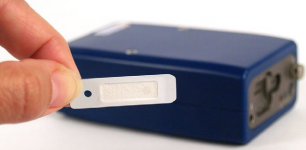
\includegraphics[scale=0.35]{microaeth}
\caption{A microaetholometer}
\label{fig:microaeth}
\end{figure}

The microaeth provides "Real-time analysis by measuring the rate of change in absorption of transmitted light due to continuous collection of aerosol deposit on filter" (\cite{Aethlabs2016}). The picture above shows one of the filters being changed, upon which particles are collected by the sucking of air by the device, and then passing this through the filter. The absorbtion of light is that